\documentclass[a4paper]{scrartcl}
% Use small margins
\usepackage[left=1.5cm, right=1.5cm, top=1cm, bottom=2cm]{geometry}
\usepackage[unicode,
            pdfencoding=auto,
            pdfinfo={
              Title={Sprawozdanie Dioda},
              Author={Maciej Mionskowski},
              Subject={Sprawozdanie Dioda},
              Keywords={},
              Producer={xelatex},
            },
]{hyperref}
\usepackage[T1]{fontenc}
\usepackage{polski}
\usepackage[polish]{babel}
\usepackage[utf8]{inputenc}
\usepackage{ upgreek }
\usepackage{array}
\usepackage{caption}
\usepackage{tabularx}
\usepackage{graphicx}
\graphicspath{ {images/} }
\renewcommand{\arraystretch}{1.5}

\author{Maciej Mionskowski}
\title{Sprawozdanie 2}
\date{}
\subtitle{Dioda półprzewodnikowa}
\begin{document}
	{\let\newpage\relax\maketitle}
	{\begin{center}Celem ćwiczeń było zapoznanie z właściwościami diody półprzewodnikowej.\end{center}}
	\begin{section}{Działanie prostownicze diody półprzewodnikowej w obwodzie elektrycznym}
		\begin{subsection}{Cel}
			Celem ćwiczenia było poznanie właściwości diody takich jak: przewodzenie prądu w jednym kierunku, zjawisko napięcia progowego $ U_{p} $ i zmierzenie go dla diody prostowniczej. 
		\end{subsection}
		\begin{subsection}{Analiza}
				\begin{figure}[ht]
				\begin{center}
					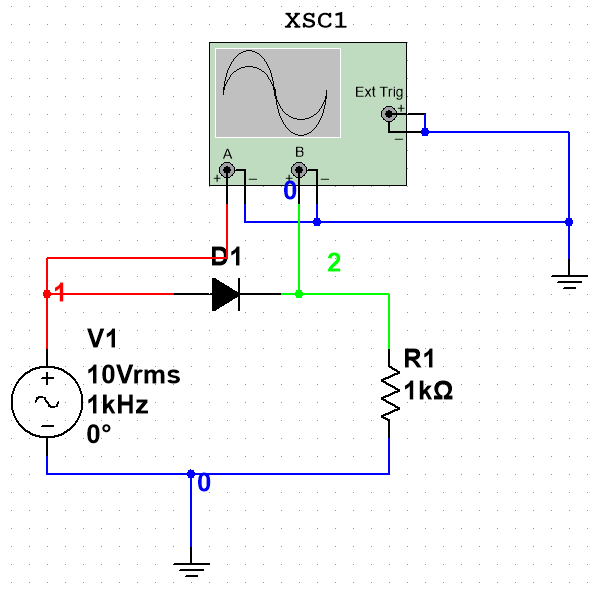
\includegraphics[width=0.4\linewidth]{exercise-1-circuit-fixed}
					\caption{Prosty obwód z diodą}
					\label{fig:circuit-1}
				\end{center}
				\end{figure}

				\begin{table}[ht]
					\caption{Wartości napięć zmierzonych w obwodzie na rysunku \ref{fig:circuit-1} }
					\begin{tabular}{| >{\bfseries}p{3.5cm} | l | l |}
						\hline
						 Wartość & \bfseries Dioda włączona jak na rys. 1 & \bfseries Dioda włączona w przeciwnym zwrocie \\ \hline
						Napięcie progowe (oscyloskop) & $ 0.722V $ & $ 0.722V $ \\ \hline
						Napiecie progowe (transient) & $ 0.722V $ & $ 0.722V $ \\ \hline
						Napiecie średnie wyprostowane & $ 4.15498V $ & $ -4.15498V $ \\ \hline

					\end{tabular}
				\end{table}

				\begin{figure}[ht]
				\begin{center}
					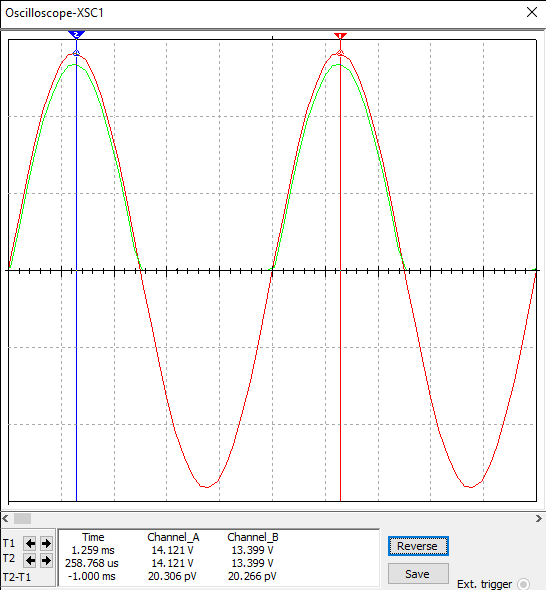
\includegraphics[width=0.6\linewidth]{exercise-1-osciloscope}
					\caption{Pomiar na oscyloskopie}
					\label{fig:circuit-1-osc}
				\end{center}
				\end{figure}

				\begin{figure}[!ht]
				\begin{center}
					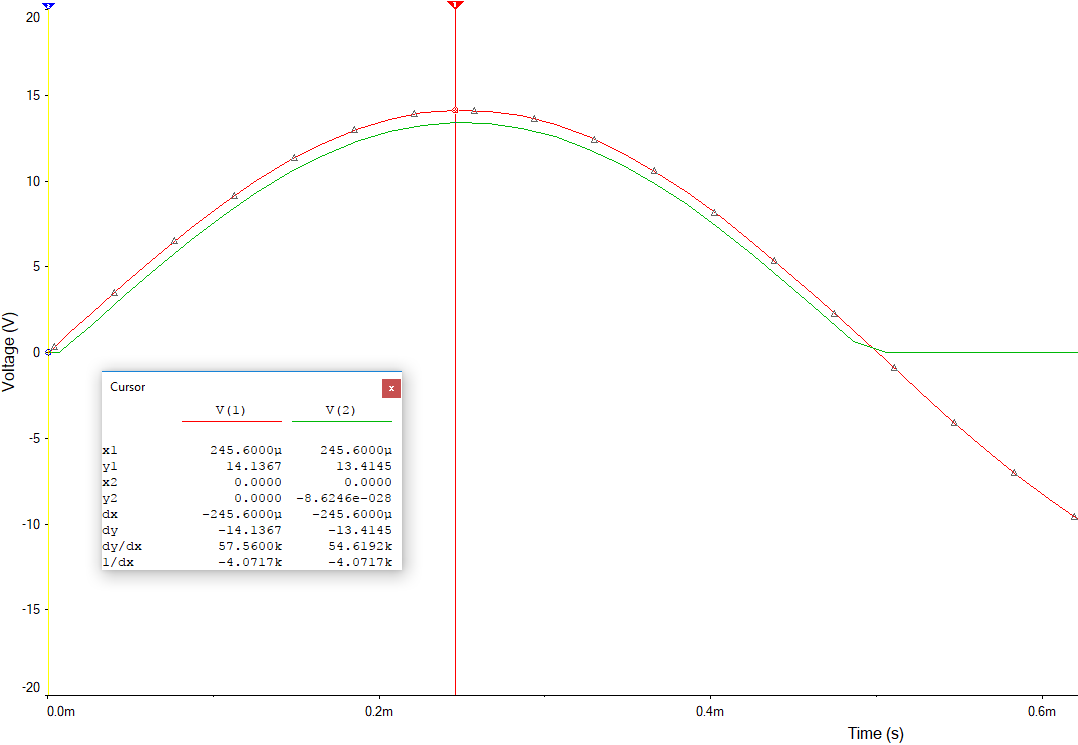
\includegraphics[width=0.7\linewidth,scale=2]{exercise-1-transient}
					\caption{Analiza transient}
					\label{fig:circuit-1-transient}
				\end{center}
				\end{figure}
		\end{subsection}
		\begin{subsection}{Wniosek}
			Z powyższej analizy wynika, że dioda posiada napięcie progowe wynoszące $\sim0.72 V $. Rozbieżności w powyższych danych spowodowane są błędem pomiarowym polegającym na: niewłaściwym ustawieniu kursorów, a także niedokładności programu MultiSim. Zarówno na analizie transient jak i na oscyloskopie możemy zauważyć, że prąd płynie tylko w jedną stronę (od $+$ do $-$).
		\end{subsection}
	\end{section}
	\begin{section}{Prostownik jednopołówkowy z filtrem RC na wyjściu}
		\begin{subsection}{Cel}
			Celem ćwiczenia było poznanie właściwości prostownika jednopołówkowego z filtrem RC, zmierzenie wartości tętnień i ich redukcja.
		\end{subsection}
		\begin{subsection}{Analiza}
				\begin{figure}[ht]
				\begin{center}
					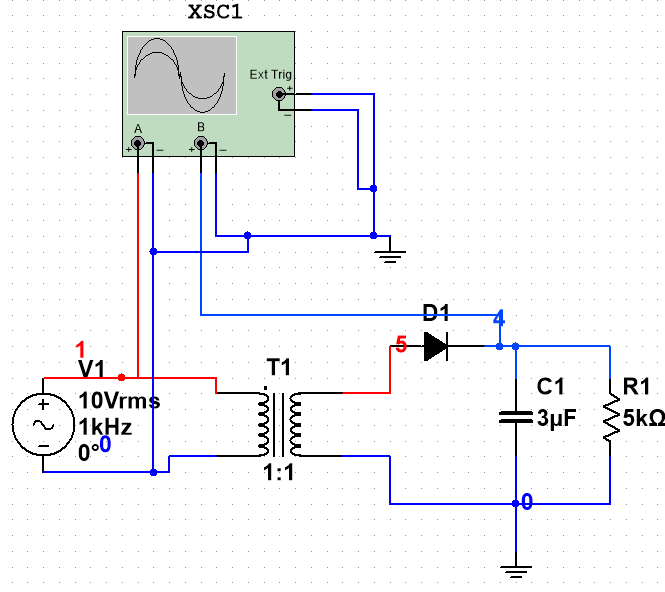
\includegraphics[width=0.8\linewidth,scale=2]{exercise-2-circuit-fixed}
					\caption{Prosty obwód z prostownikiem jednopołówkowym}
					\label{fig:circuit-2}
				\end{center}
				\end{figure}

				\begin{table}[ht]
					\begin{center}
					\caption{Wartości napięć zmierzonych w obwodzie na rysunku \ref{fig:circuit-2} }
					\begin{tabular}{| >{\bfseries}p{4.5cm} | l | l | l | l |}
						\hline
						$ R_{1} $ & $ 5k\Omega $ & $ 5k\Omega $ & $ 5k\Omega $ & $ 5k\Omega $ \\ \hline
						$ C_{1} $ & brak & $1 \upmu F$ & $3 \upmu F$ & $1.6\upmu F$ \\ \hline \hline
					
						Napięcie tętnień $U_{t} [V] $ (transient)  & $ 13.43V $ & $ 2.17V $ & $ 0.7863V $ & $ 1.33V $\\ \hline


					\end{tabular}
					\end{center}
				\end{table}
				\pagebreak
				\begin{figure}[h]
				\begin{center}
					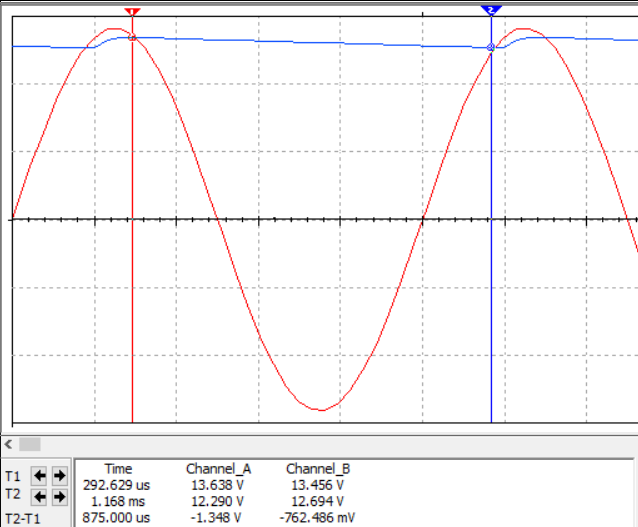
\includegraphics[width=0.6\linewidth,scale=2]{exercise-2-osciloscope}
					\caption{Pomiar na oscyloskopie dla $C_{1} = 3\upmu F$}
					\label{fig:circuit-2-osc}
				\end{center}
				\end{figure}
				\begin{figure}[!ht]
				\begin{center}
					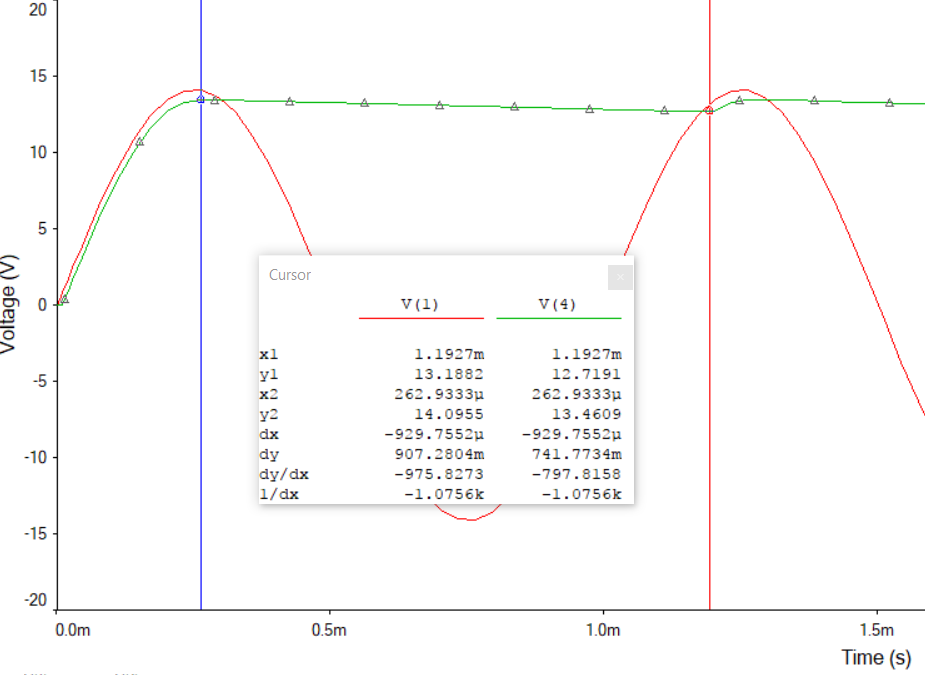
\includegraphics[width=0.8\linewidth,scale=2]{exercise-2-transient}
					\caption{Analiza transient dla $C_{1} = 3\upmu F$}
					\label{fig:circuit-2-transient}
				\end{center}
				\end{figure}
		\end{subsection}
		\begin{subsection}{Wniosek}
			Analiza pokazuje, że dodanie kondensatora powoduje zaczęcie występowania napięcia tętnień. Zwiększenie pojemności kondensatora powoduje zmniejszenie napięcia tętnień. Analogicznie czym mniejsza pojemność kondensatora tym tętnienia są większe. Dzieje się tak dlatego, że podczas gdy negatywna część napięcia nie jest przetwarzana kondensator oddaje ładunki. Czym większa pojemność tym więcej ich może oddać.
		\end{subsection}
	\end{section}
	\begin{section}{Prostownik w układzie Graetza}
		\begin{subsection}{Cel}
			Celem ćwiczenia było poznanie zasady działania i zmierzenia wartości napięcia tętnień układu z prostownikiem dwupołówkowym - układem Graetza.
		\end{subsection}
		\begin{subsection}{Analiza}
				\begin{figure}[ht]
				\begin{center}
					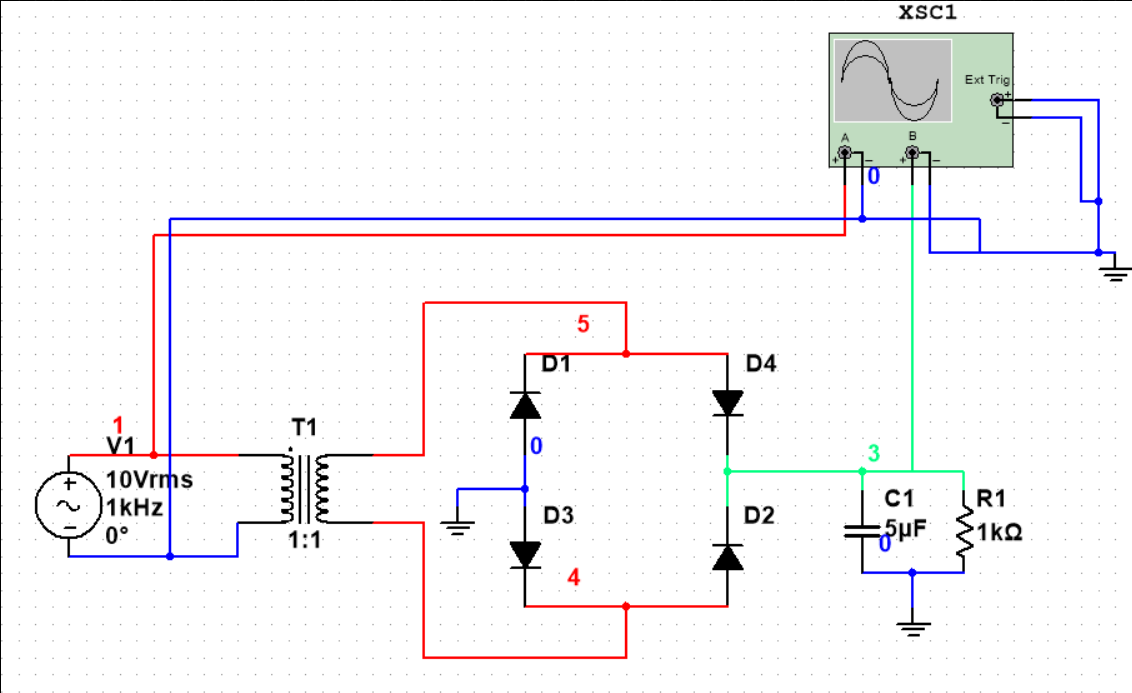
\includegraphics[width=0.5\linewidth,scale=2]{exercise-3-circuit}
					\caption{Obwód z prostownikiem Graetza}
					\label{fig:circuit-3}
				\end{center}
				\end{figure}

				\begin{table}[ht]
					\begin{center}
					\caption{Wartości napięć zmierzonych w obwodzie na rysunku \ref{fig:circuit-3} }
					\label{table:circuit-3}
					\begin{tabular}{| >{\bfseries}p{4.5cm} | l | l | l | l |}
						\hline
						$ R_{1} $ & $ 1k\Omega $ & $ 1k\Omega $ & $ 1k\Omega $ & $ 10k\Omega $ \\ \hline
						$ C_{1} $ & brak & $5 \upmu F$ & $2 \upmu F$ & $5\upmu F$ \\ \hline \hline
					
						Napięcie tętnień $U_{t} [V] $ (transient)  & $ 12.645V $ & $ 0.9547V $ & $ 2.1533V $ & $ 0.1029V $\\ \hline


					\end{tabular}
					\end{center}
				\end{table}
				\begin{figure}[h]
				\begin{center}
					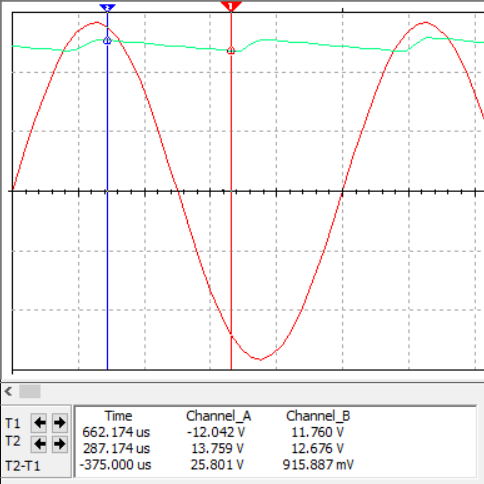
\includegraphics[width=0.39\linewidth,scale=2]{exercise-3-osciloscope}
					\caption{Pomiar na oscyloskopie dla $C_{1} = 5\upmu F$}
					\label{fig:circuit-3-osc}
				\end{center}
				\end{figure}
				\pagebreak
				\begin{figure}[!ht]
				\begin{center}
					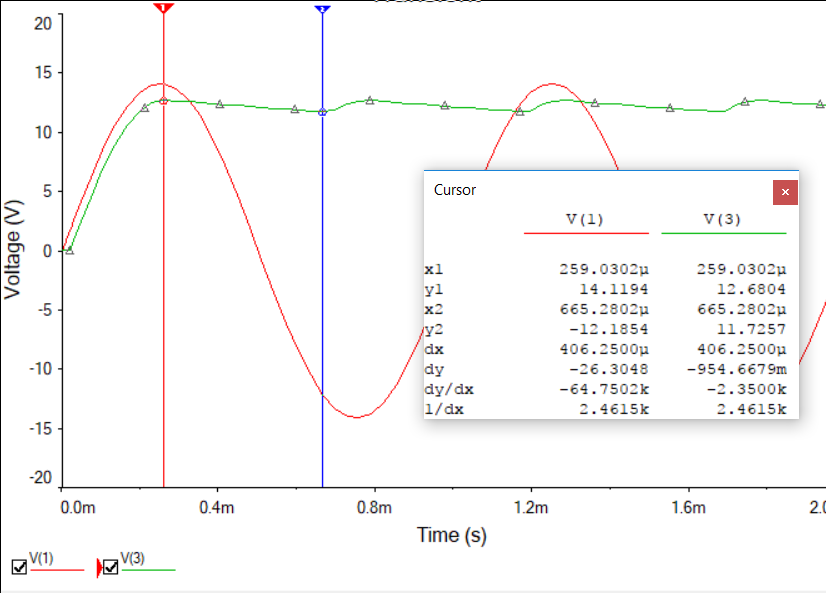
\includegraphics[width=0.7\linewidth,scale=2]{exercise-3-transient}
					\caption{Analiza transient dla $C_{1} = 5\upmu F$}
					\label{fig:circuit-3-transient}
				\end{center}
				\end{figure}
				\begin{figure}[!ht]
				\begin{center}
					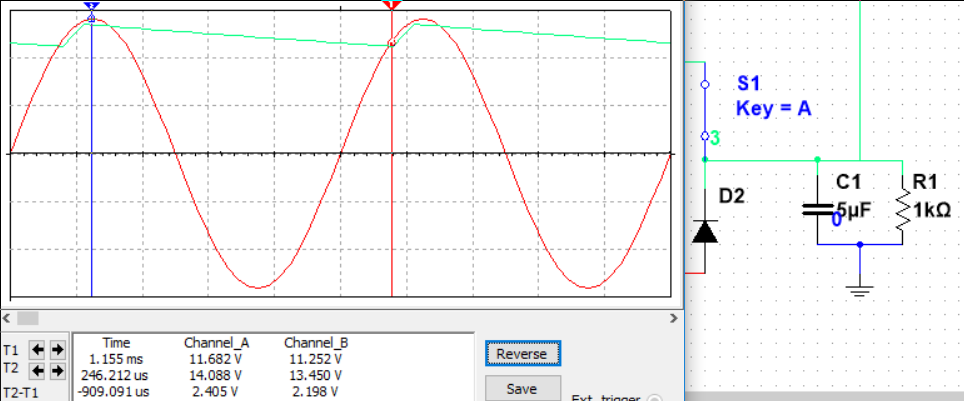
\includegraphics[width=0.7\linewidth,scale=2]{exercise-3-diode-fail}
					\caption{Pomiar na oscyloskopie dla uszkodzonej diody (\textit{7a}) przy $C_{1} = 5\upmu F$}
				\end{center}
				\end{figure}
				\begin{figure}[!ht]
				\begin{center}
					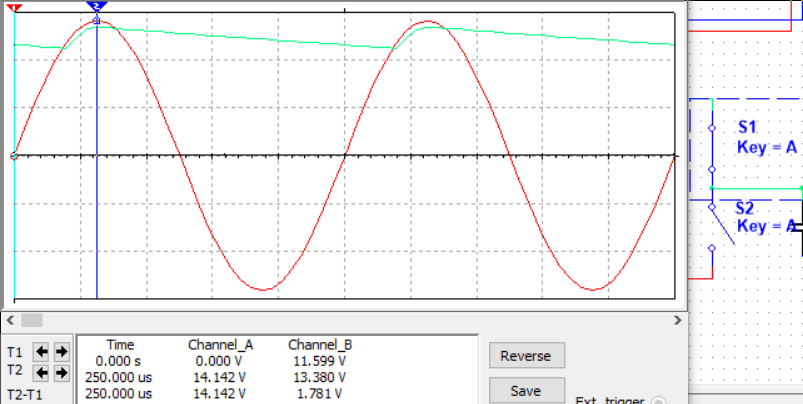
\includegraphics[width=0.7\linewidth,scale=2]{exercise-3-diode-fail-2}
					\caption{Pomiar na oscyloskopie dla uszkodzonych diód (\textit{7b}) przy $C_{1} = 5\upmu F$}
				\end{center}
				\end{figure}
				\begin{figure}[!ht]
				\begin{center}
					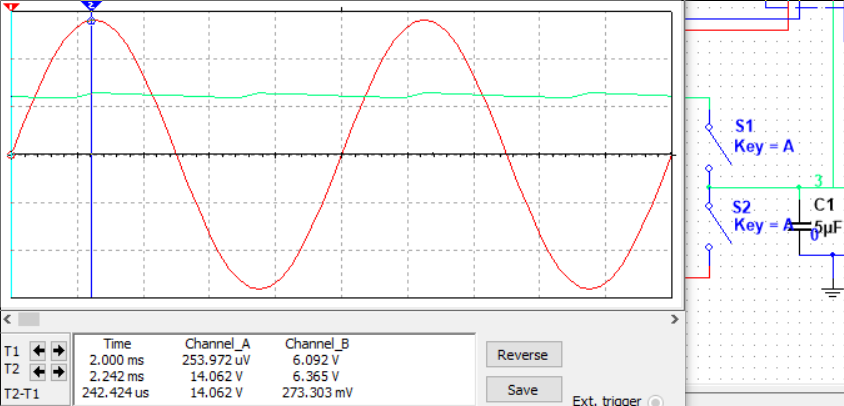
\includegraphics[width=0.7\linewidth,scale=2]{exercise-3-diode-fail-3}
					\caption{Pomiar na oscyloskopie dla uszkodzonych diód (\textit{7c}) przy $C_{1} = 5\upmu F$}
				\end{center}
				\end{figure}

		\end{subsection}
		\pagebreak
		\begin{subsection}{Wniosek}
			Mostek Graetza prostuje obie połówki ($-$, $+$) prądu zmiennego, można to zaobserwować przy analizie tętnień na rysunku \ref{fig:circuit-3-transient}. W przeciwieństwie do prostownika jednopołówkowego, przy mostku Graetza występują dwa tętnienia na okres sinusoidy.Można też zauważyć, że napięcie progowe $U_{p} $ liczone jest teraz dwukrotnie. Oznacza to, że w jednym momencie prąd płynie tylko przez dwie diody. Podobnie jak przy prostowniku jednopołówkowym, wzrost pojemności kondensatora powoduje zmniejszenie napiecia tętnień $U_{t}$. Wraz ze wzrostem rezystancji napięcie tętnień również maleje, ponieważ kondensator wolniej się rozładowuje. Z tablicy \ref{table:circuit-3} można również wywnioskować, że pojemność kondensatora nie jest liniowo skorelowana z napięciem tętnień $U_{t}$. Różne uszkodzenia mostka Graetza wpływają niekorzystnie na jego działanie.
		\end{subsection}
	\end{section}
	\begin{section}{Detektor szczytowy}
		\begin{subsection}{Cel}
			Celem ćwiczenia było zapoznanie z zasadą działania detektora szczytowego.
		\end{subsection}
		\begin{subsection}{Analiza}
				\begin{figure}[ht]
				\begin{center}
					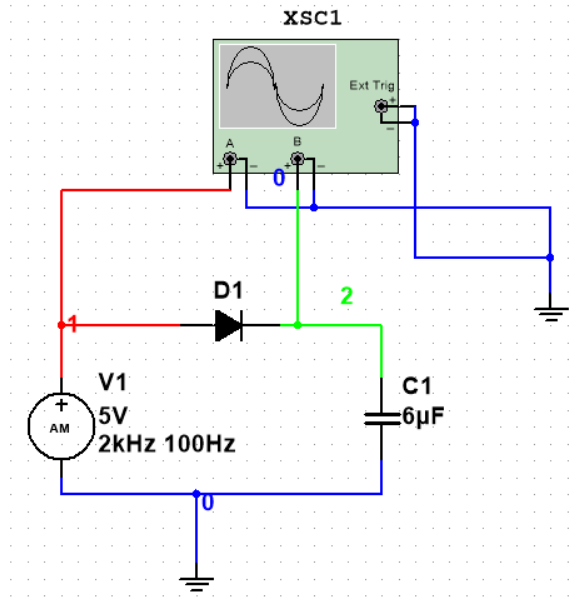
\includegraphics[width=0.4\linewidth]{exercise-4-circuit}
					\caption{Prosty detektor szczytowy}
					\label{fig:circuit-4}
				\end{center}
				\end{figure}

				\begin{figure}[!ht]
				\begin{center}
					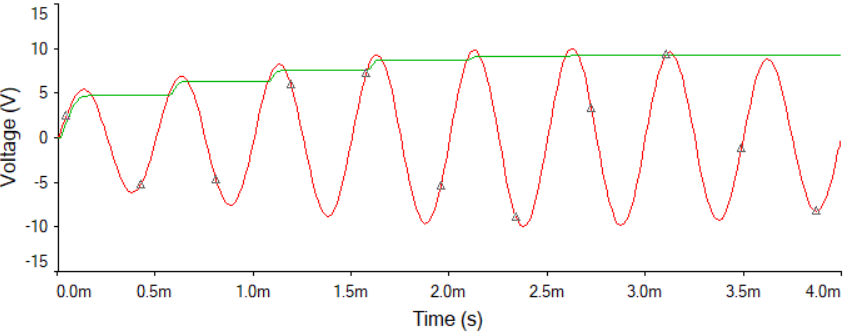
\includegraphics[width=\linewidth]{exercise-4-transient}
					\caption{Analiza transient}
					\label{fig:exercise-4-transient}
				\end{center}
				\end{figure}
		\end{subsection}
		\begin{subsection}{Wniosek}
			Ze schematu obwodu \ref{fig:circuit-4} oraz analizy transient tego obwodu na rysunku \ref{fig:exercise-4-transient} można wywnioskować jak działa detektor szczytowy. Widać, że napięcie na kondensatorze wynosi niemal tyle ile wynosiła maksymalna wartość napięciai do tej pory - różnica spowodowana jest napięciem progowym diody $ U_{p} = 0.72V $. Zasada działania detektora jest prosta, podczas dodatniego i większego niż obecnie na kondensatorze przebiegu napięcia wejścia dioda przewodzi prąd ładując kondensator. Przy napięciu mniejszym niż obecnie na kondensatorze prąd nie może się \textit{cofnąć} do źródła, ponieważ dioda jest polaryzowana zaporowo, sprawia to, że napięcie na kondensatorze może tylko wzrosnąć.
		\end{subsection}
	\end{section}
	\begin{section}{Demodulator diodowy}
		\begin{subsection}{Cel}
			Celem ćwiczenia było zapoznanie z zasadą działania detektora szczytowego.
		\end{subsection}
		\begin{subsection}{Analiza}
				\begin{figure}[ht]
				\begin{center}
					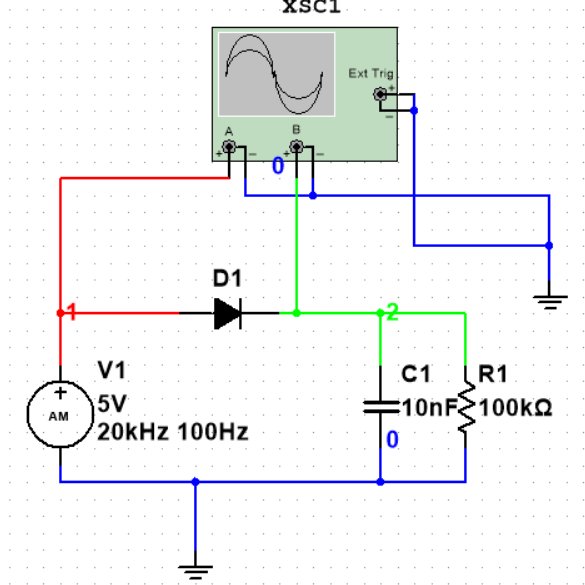
\includegraphics[width=0.4\linewidth]{exercise-5-circuit}
					\caption{Prosty demodulator AM z podłączonym oscyloskopem}
					\label{fig:circuit-5}
				\end{center}
				\end{figure}

				\begin{figure}[!ht]
				\begin{center}
					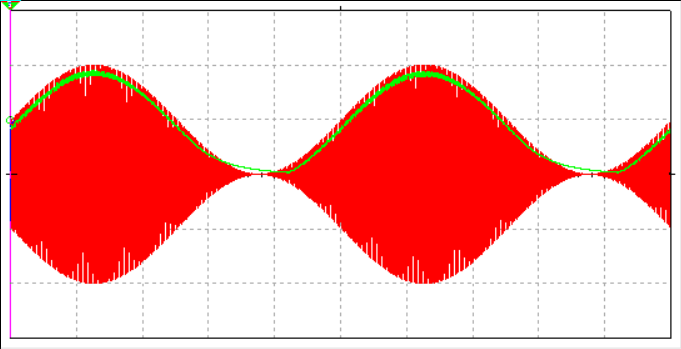
\includegraphics[width=0.7\linewidth]{exercise-5-100k}
					\caption{Pomiar na oscyloskopie przy $R_{1} = 100k\Omega$}
					\label{fig:exercise-5-100k}
				\end{center}
				\end{figure}
				\begin{figure}[!ht]
				\begin{center}
					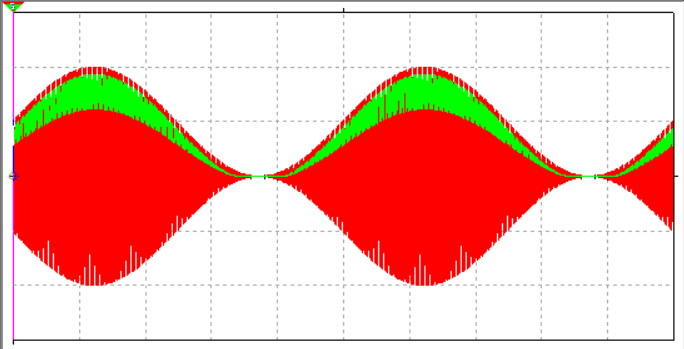
\includegraphics[width=0.7\linewidth]{exercise-5-10k}
					\caption{Pomiar na oscyloskopie przy $R_{1} = 10k\Omega$}
					\label{fig:exercise-5-10k}
				\end{center}
				\end{figure}
				\begin{figure}[!ht]
				\begin{center}
					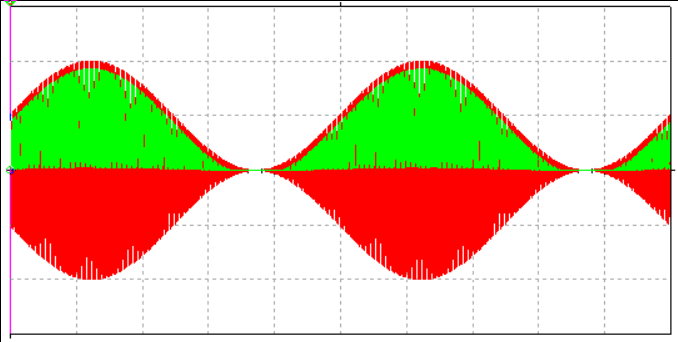
\includegraphics[width=0.7\linewidth]{exercise-5-1k}
					\caption{Pomiar na oscyloskopie przy $R_{1} = 1k\Omega$}
					\label{fig:exercise-5-1k}
				\end{center}
				\end{figure}
		\end{subsection}
		\clearpage
		\begin{subsection}{Wniosek}
			Zasada działania demodulatora AM jest bardzo podobna i bazuje na działaniu detektora szczytowego. Różnicą jest dodatkowy opornik, który ma za zadanie częściowo rozładować kondensator, tak aby kolejny grzbiet fali mógł zostać zarejestrowany jako szczyt. Ważny jest tutaj odpowiedni dobór opornika i kondensatora. Można zauważyć, że przy $R_{1} = 100k\Omega$ (rysunek \ref{fig:exercise-5-100k}), demodulator zachowuje się poprawnie. Natomiast przy mniejszych oporach \ref{fig:exercise-5-10k} i \ref{fig:exercise-5-1k} sygnał nie jest poprawnie demodulowany (kondensator jest za bardzo rozładowywany) i powstają skoki. Demodulacja AM polega na wydobyciu oryginalnej informacji z fali. Ma zostosowanie między innymi w radiotelekomunikacji.
		\end{subsection}
	\end{section}
\end{document}
